\documentclass{article}
\usepackage{neb-titles}
\usepackage{neb-formulas}
\usepackage{flexfig}

\usepackage{graphicx}


\begin{document}

\TestTitle[class={College Algebra}, name={Test 3}, term={Spring}, date={Oct. 19}, year={2015}, form={A}]

\AlgebraFacts[geom={show}]

\begin{enumerate}
\item Fill in the boxes to describe the long-term behavior of the following polynomial. \[ p(x) = 3x^3 - 2x + 1 \].

\begin{itemize}
\item As $x \rightarrow \infty$, $p(x) \rightarrow$ \framebox(30,20){} \vspace{0.5cm}
\item As $x \rightarrow -\infty$, $p(x) \rightarrow$ \framebox(30,20){}
\end{itemize} \vspace{1cm}

\item The polynomial \[ p(x) = x^5 - 5x^4 - 3x^3 + 29x^2 + 2x - 24 \] has roots at ${-1;3;-2;1}$. Completely factor $p(x)$ as a product of linear factors. \vspace{6cm}

\item Construct a polynomial of degree 3 which has roots at -1, 1, and 2. \vspace{5cm}

\newpage

\item The polynomial \[ p(x) = x^4 - 3x^3 + 6x - 4 \] has a root at $\sqrt{2}$. Completely factor $p(x)$ as a product of linear factors. \vspace{9cm}

\item Complete the square to find the standard form of the folloing parabola. \[ y = x^2 + 8x + 18 \] \vspace{6cm}

\item Find an equation for the parabola with horizontal directrix having vertex $(4, -7)$ and focal length -1. \vspace{2cm}

\newpage

\item Find the domain of the following rational function. \[ f(x) = \frac{x^2 + x - 2}{x^3 - 5x^2 + 8x - 4} \] \vspace{5cm}

\item Plot the following ellipse in the space provided. \[ \left(\frac{x + 5}{4}\right)^2 + \left(\frac{y - 7}{2}\right)^2 = 1 \]

\begin{center}
\CartesianPlane[axes=yes,h=10,w=10]
\end{center} \vspace{1cm}

\newpage

\item Find the long-term behavior asymptote of the following rational function. \[ f(x) = \frac{x^3 + x^2 - 9x - 9}{x - 6} \] \vspace{6cm}

\item Plot the following parabola in the space provided. \[ y = \frac{1}{-4} \left(x - 4\right)^2 -3 \]

\begin{center}
\CartesianPlane[axes=yes,h=10,w=10]
\end{center} \vspace{1cm}

\newpage

\item Suppose you and your friends create a catapult and launch a coconut with it.
\begin{enumerate}
\item The height of the coconut $t$ seconds after launch is given by $f(t)=128t-16t^2$. How long will the coconut be in the air? (Here we assume it will hit the ground when the height is $0$).
\vspace{1in}
\item Viewing a graph of this function below, estimate the maximum height the coconut achieves. \vspace{.25in}\\ 
Maximum Height: \\ \vspace{.25in}
\begin{center}
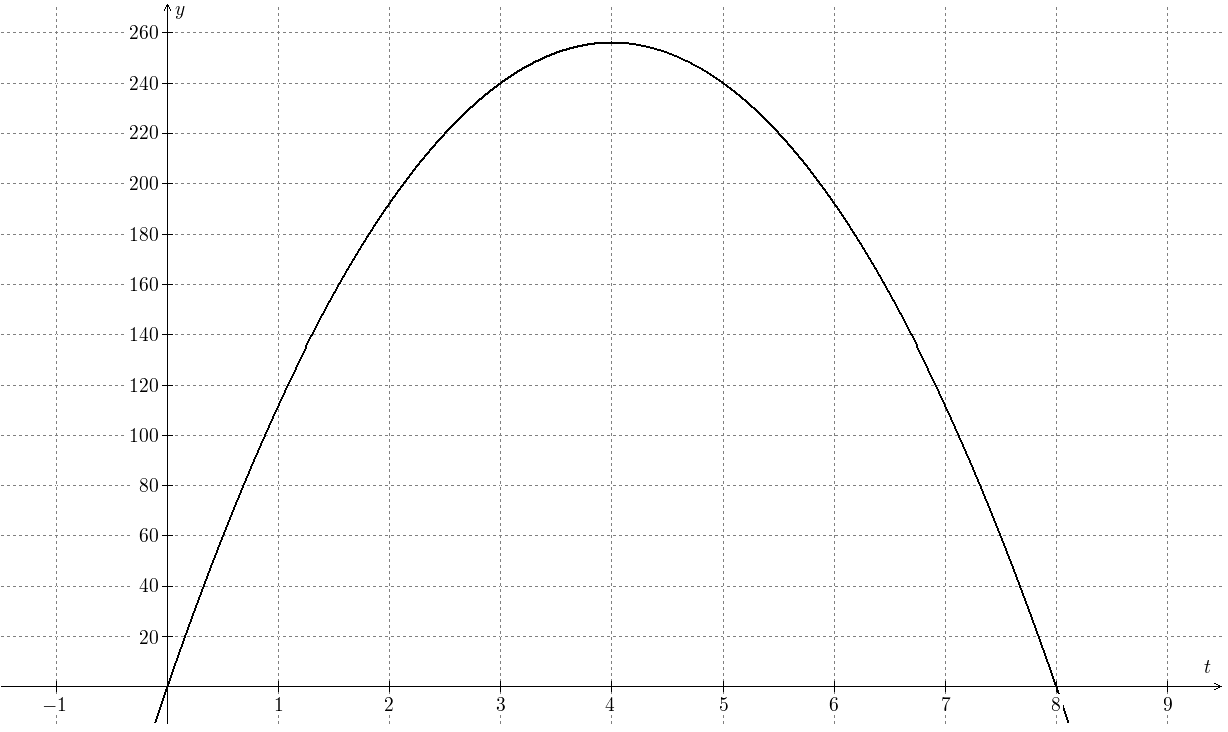
\includegraphics[scale=.5]{ca/tex/coconut.png}
\end{center}
\item Recalling that the function of the height of the coconut is $f(t)=128t-16t^2$, use your knowledge about quadratic functions to determine the actual maximum height the coconut achieves.
\end{enumerate}
\end{enumerate}

\end{document}
